
\documentclass[polish,12pt]{aghthesis}

\usepackage[utf8]{inputenc}
\usepackage{url}
\usepackage{hyperref}
\usepackage{pgffor}

\usepackage{natbib}
\usepackage{keyval}
\usepackage{usebib}
\usepackage{pdfpages}
\bibinput{bibliografia}

\graphicspath{{images/}}

\renewcommand*{\figureautorefname}{Rys.}
\renewcommand*{\subsectionautorefname}{rozdziale}

\author{Wojciech Baszczyk}

\title{Wysokopoziomowy interfejs do zarządzania urządzeniami internetu rzeczy}

\supervisor{dr inż.\ Włodzimierz Funika}

\date{2016}

% Szablon przystosowany jest do druku dwustronnego
\begin{document}

\maketitle

\tableofcontents
\newpage

\foreach \secf in {
	section1.tex
	% section2.tex,
	% section3.tex,
	% section4.tex,
	% section5.tex
	} {
	\input{sections/\secf}
	\newpage
}

% \nocite{genetic-wiki, otp-www}

\bibliography{bibliografia}
\newpage

\listoffigures
\newpage


\appendix


\section{Załączniki - KU KDM '16}

\subsection{Abstrakt}
\begin{figure}[!htbp]
	\centering
	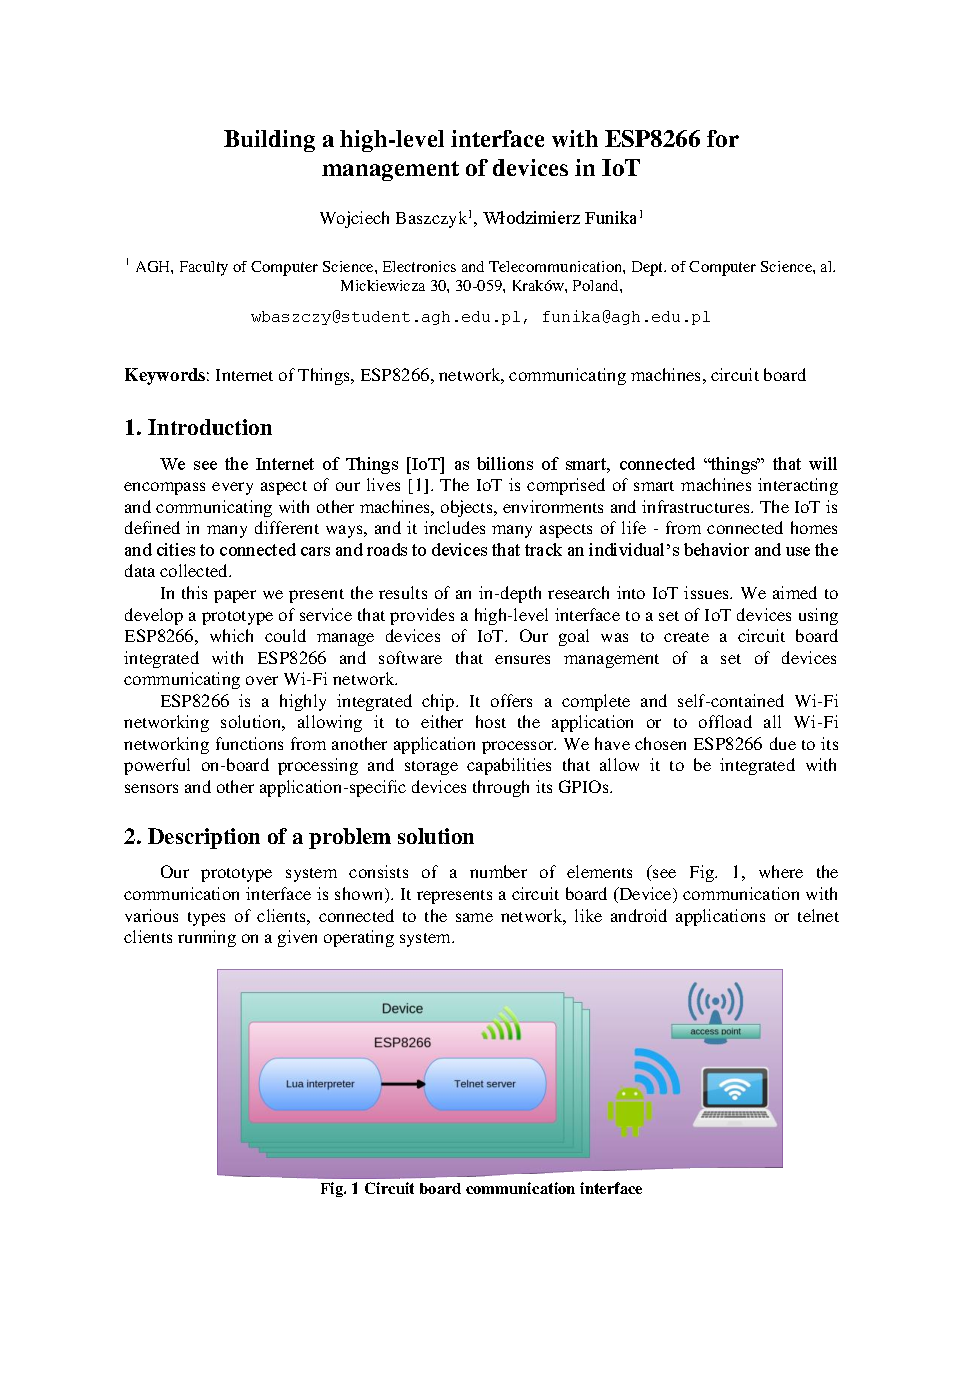
\includegraphics[page=1,width=0.9\textwidth]{{include/KUKDM2016-WB-v0.6}.pdf}
	\caption{Abstrakt przesłany na KU KDM '16. Strona 1.}
	\label{app:kdm14-abstr01}
\end{figure}
\begin{figure}[!htbp]
	\centering
	\includegraphics[page=2,width=0.9\textwidth]{{include/KUKDM2016-WB-v0.6}.pdf}
	\caption{Abstrakt przesłany na KU KDM '16. Strona 2.}
	\label{app:kdm14-abstr02}
\end{figure}

\subsection{Poster}
\begin{figure}[!htbp]
	\centering
	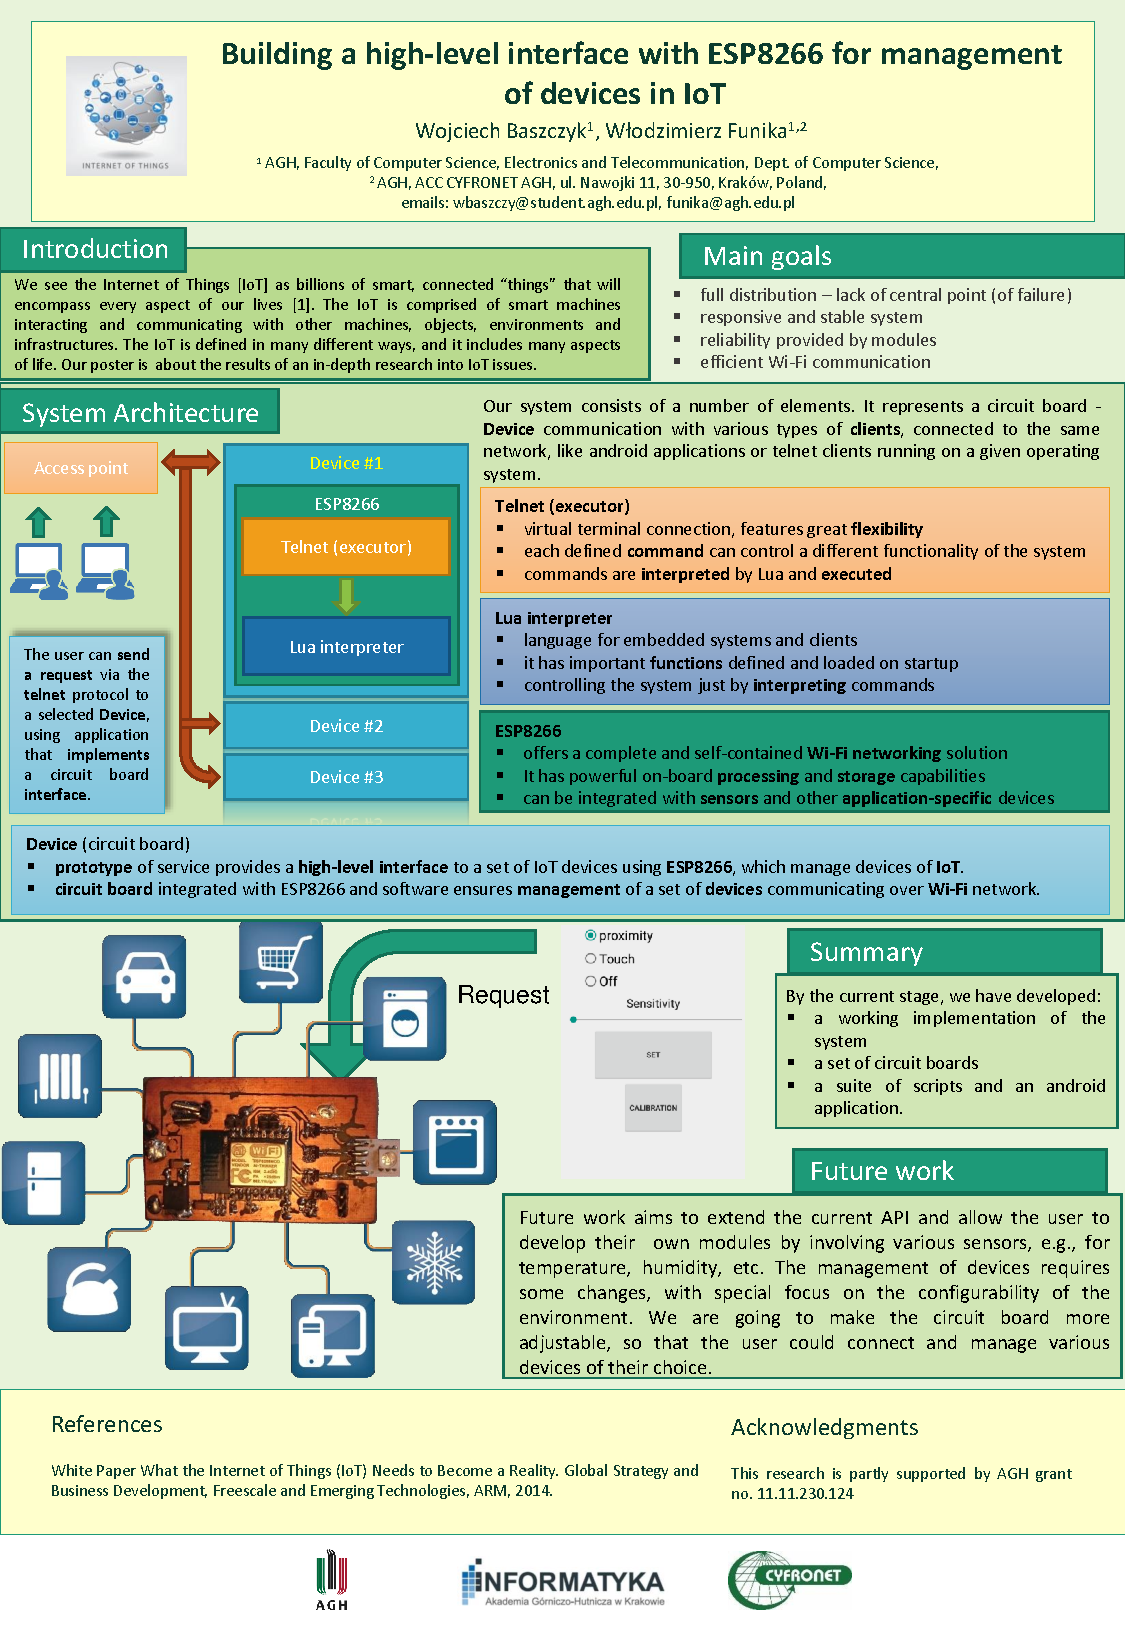
\includegraphics[page=1,width=.9\textwidth]{include/WB-WF-poster_v05e.pdf}
	\caption{Poster zaprezentowany na KU KDM '16.}
	\label{app:kdm14-poster}
\end{figure}


\newpage

\end{document}
